\documentclass{article}

\usepackage{amsmath}
\usepackage{graphicx}

\newcommand{\rr}{\mathbf{r}}
\newcommand{\ii}{\mathbf{i}}
\newcommand{\jj}{\mathbf{j}}
\newcommand{\kk}{\mathbf{k}}

\DeclareMathOperator{\curl}{curl}

\begin{document}

{\bf Quiz \#13; Tuesday, date: 04/24/2018}

{\bf MATH 53 Multivariable Calculus with Stankova}

{\bf Section \#117; time: 5 -- 6:30 pm}

{\bf GSI name: Kenneth Hung}

{\bf Student name:}

\vspace*{0.25in}

\begin{enumerate}
\item Find the area of the part of the paraboloid $z = x^2 + y^2$ that lies within the cylinder $x^2 + y^2 = 1$.

\item {\em True / False?} Recall that the integral
\[
\int_C \frac{-y \ii + x \jj}{x^2 + y^2} \cdot d\rr = 2\pi
\]
for any positive oriented simple closed path that encloses the origin. The integral along one loop of the following path is also $2\pi$.
\begin{center}
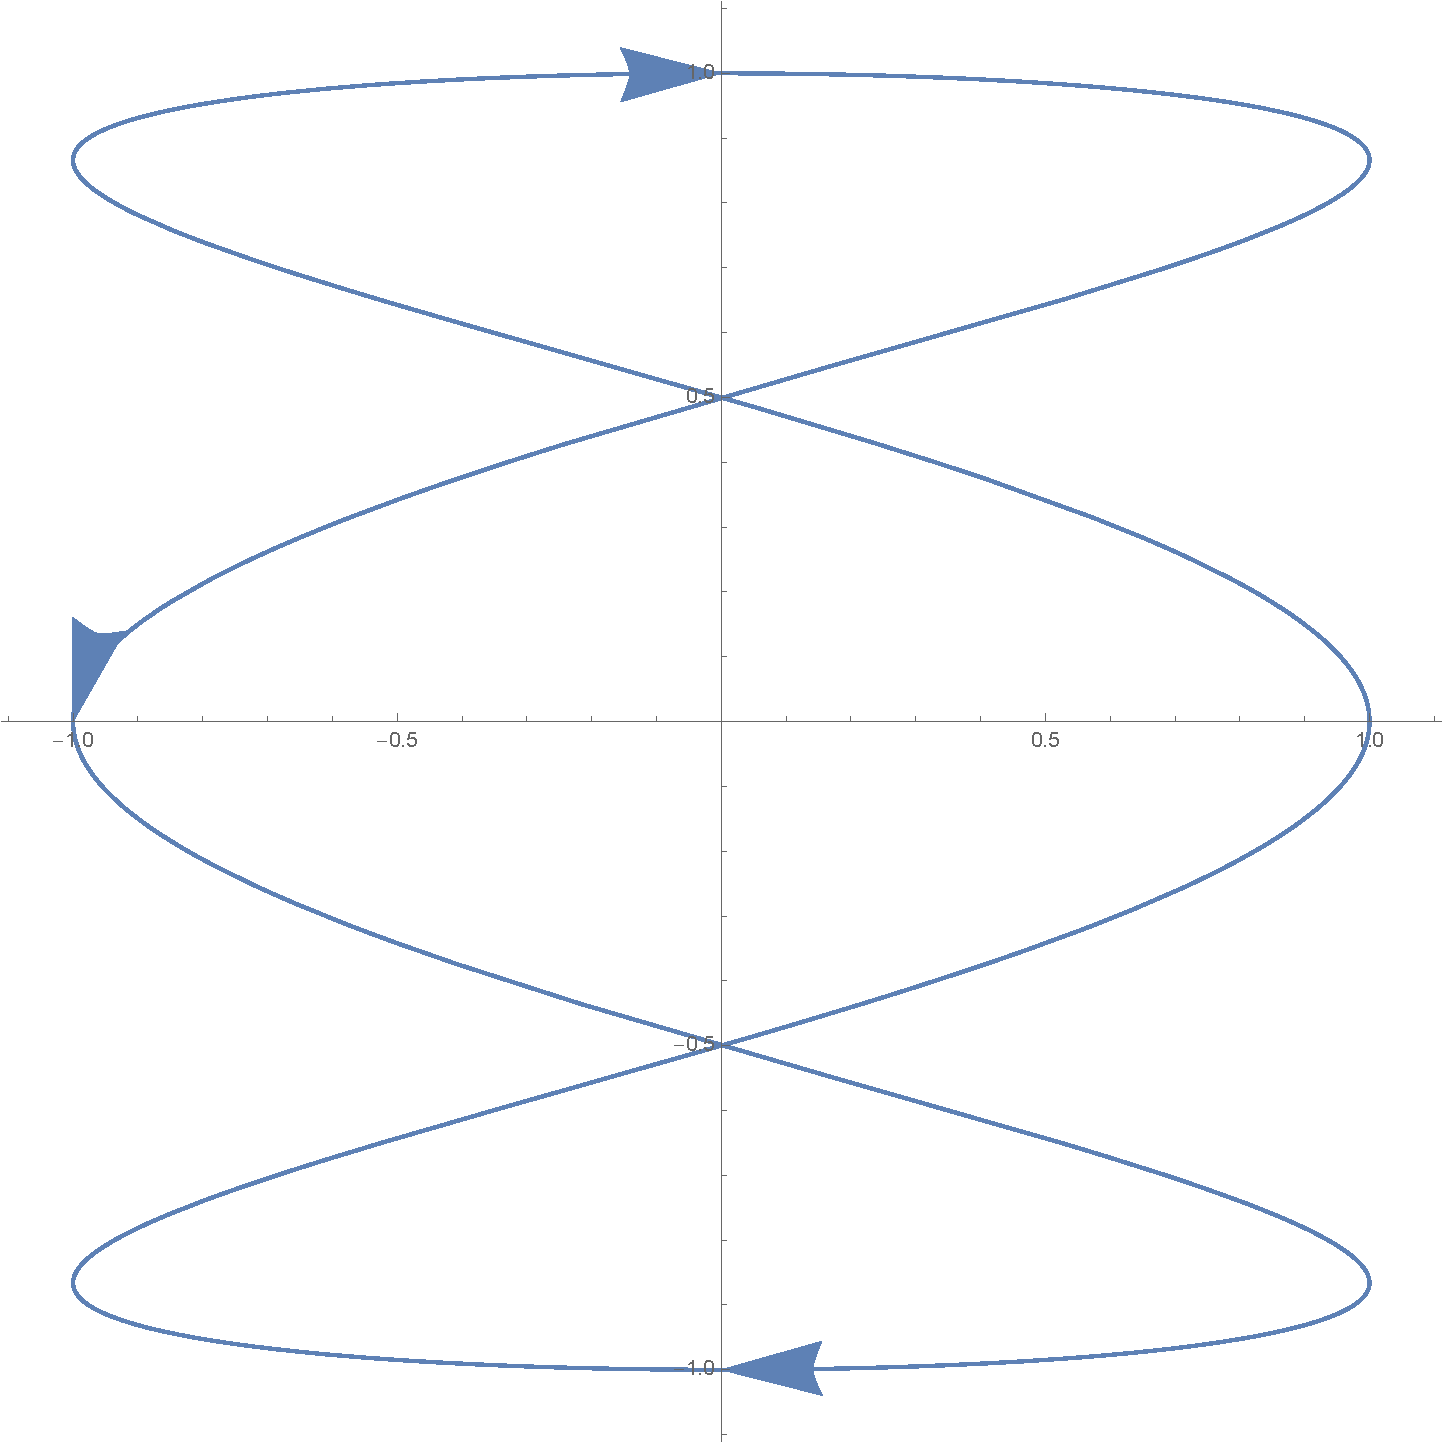
\includegraphics[width=0.5\textwidth]{quiz13dis117pic}
\end{center}

\item {\em True / False?} For any single functions $f$, $g$, $h$ that are smooth and have continuous derivatives, there is a vector field $\mathbf{G}$ such that $\curl \mathbf{G} = \langle f'(y), g'(z), h'(x) \rangle$.
\end{enumerate}

\end{document}